\section{Theoretische Grundlagen}
\label{sec:theoretische_grundlagen}

Bei dem Debye-Scherrer-Verfahren handelt es sich um eine Methode der Strukturaufklärung.
Mithilfe eines monochromatischen Röntgenstrahls wird eine kristalline Probe bestrahlt, welche zu einer Beugung des Strahls führt.
Aus dem entstehenden Interferenzmuster lässt sich nun die Struktur des Gitters und die Gitterkonstante berechnen.
In diesem Versuch wird ein Metall, im Folgenden Probe 6 genannt, und ein Salz, im Folgenden Salz 1 genannt, untersucht.

\subsection{Beschreibung der Kristallstruktur} % (fold)
\label{sub:subsection_name}

Eine Kristallstruktur besteht aus einem Gitter und einer Basis.
Dabei beschreibt diese die Faltung der beiden Bestandteile und ist somit vollständig bekannt, wenn das Gitter und die Gestalt der Basis bekannt ist.
Das Gitter kann nun über die fundamentalen Translationen $\vec{a}$, $\vec{b}$ und $\vec{c}$ aufgespannt werden, sodass jeder Punkt durch einen Vektor
\begin{equation*}
    \vec{t} = n_1 \vec{a} + n_2 \vec{b} + n_3 \vec{c} \qquad n_1, n_2, n_3 \in \mathbb{Z}\,,
\end{equation*}
beschrieben werden kann (Abb. \ref{fig:fund_trans}).

\begin{figure}[h!]
    \centering
    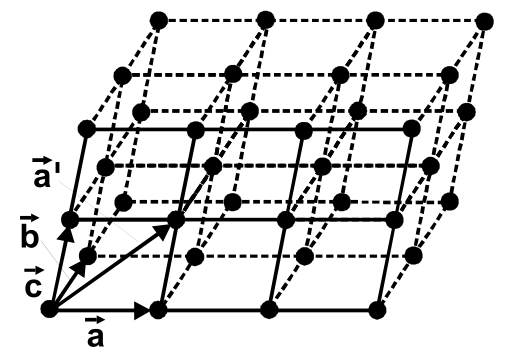
\includegraphics[width=0.5\linewidth]{images/fund_trans.png}
    \caption{Erzeugung eines Punktgitters mithilfe der fundamentalen Translation $\vec{a}$, $\vec{b}$ und $\vec{c}$ \cite{V41}.}
    \label{fig:fund_trans}
\end{figure}

Die kleinste Einheit der Struktur ist die Elementarzelle, welche durch das Parallelpiped des Vektors $\vec{t}$ aufgespannt wird.
Teilt möglichen Elementarzellen in ihre Symmetrieeigenschaften auf, so ergeben sich in 3 Dimensionen 14 verschiedene Möglichkeiten.
Diese werden als Bravais-Gitter bezeichnet.
In diesem Versuch werden nur kubische Systeme behandelt, welche sich in die FCC-, BCC-, und SC-Struktur unterteilen.

\subsection{Kubische Kristallstrukturen} % (fold)
\label{sub:kubische_kristallstrukturen}

Wie in Kapitel \ref{sub:subsection_name} beschrieben, bestehen kubische Systeme aus der FCC-, BCC-, und SC-Struktur.
Die kubisch-primitive Struktur (SC) besitzt die fundamentale Translation
\begin{equation*}
    \left(0, 0, 0\right)\,.
\end{equation*}
Die kubisch-raumzentrierte Struktur (BCC) hingegen hat die fundamentale Translation
\begin{equation*}
    \left(0, 0, 0\right)\, \text{und}\, \left(\frac{1}{2}, \frac{1}{2}, \frac{1}{2}\right)\,
\end{equation*}
und die kubisch-flächenzentrierte Struktur (FCC)
\begin{equation*}
    \left(0, 0, 0\right),\, \left(\frac{1}{2}, \frac{1}{2}, 0\right),\, \left(\frac{1}{2}, 0, \frac{1}{2}\right)\, \text{und}\, \left(0, \frac{1}{2}, \frac{1}{2}\right)\,.
\end{equation*}
Ein Beispiel für eine kubisch-flächenzentrierte Elementarzelle mit fundamentale Translation ist in Abbildung \ref{fig:FCC} dargestellt.
\begin{figure}[h!]
    \centering
    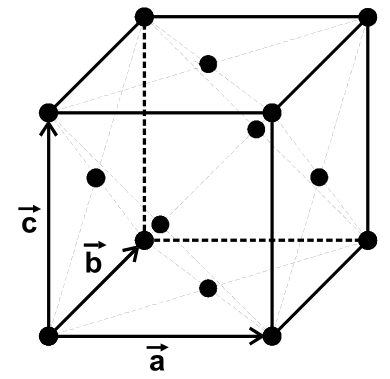
\includegraphics[width=0.5\linewidth]{images/fcc.png}
    \caption{Elementarzelle eines kubisch-flächenzentrierten Gitters \cite{V41}.}
    \label{fig:FCC}
\end{figure}
\\
Werden kubisch-flächenzentrierte Gitter kombiniert, so ergeben sich weitere Möglichkeiten.
Die Diamant-Struktur besteht aus zwei kubisch-flächenzentrierten Gittern, welche um ein Viertel der Raumdiagonalen gegeneinander versetzt sind.
Somit ergibt sich für die fundamentale Translation
\begin{equation*}
    \left(0, 0, 0\right),\, \left(\frac{1}{2}, \frac{1}{2}, 0\right),\, \left(\frac{1}{2}, 0, \frac{1}{2}\right),\, \left(0, \frac{1}{2}, \frac{1}{2}\right),\, \left(\frac{1}{4}, \frac{1}{4}, \frac{1}{4}\right),\, \left(\frac{3}{4}, \frac{3}{4}, \frac{1}{4}\right),\, \left(\frac{3}{4}, \frac{1}{4}, \frac{3}{4}\right)\, \text{und} \left(\frac{1}{4}, \frac{3}{4}, \frac{3}{4}\right)\,.
\end{equation*}

Werden die beiden Gitter durch verschiedene Atomarten besetzt, so wird von der Zinkblende-Struktur gesprochen mit den fundamentale Translation
\begin{align*}
    \text{A}&:\, \left(0, 0, 0\right),\, \left(\frac{1}{2}, \frac{1}{2}, 0\right),\, \left(\frac{1}{2}, 0, \frac{1}{2}\right)\, \text{und}\, \left(0, \frac{1}{2}, \frac{1}{2}\right),\, \\
    \text{B}&:\, \left(\frac{1}{4}, \frac{1}{4}, \frac{1}{4}\right),\, \left(\frac{3}{4}, \frac{3}{4}, \frac{1}{4}\right),\, \left(\frac{3}{4}, \frac{1}{4}, \frac{3}{4}\right)\, \text{und} \left(\frac{1}{4}, \frac{3}{4}, \frac{3}{4}\right)\,.
\end{align*}

Sind die Gitter um eine halbe Raumdiagonale verschoben, so ergibt sich die Steinsalz Struktur mit den fundamentale Translation
\begin{align*}
    \text{A}&:\, \left(0, 0, 0\right),\, \left(\frac{1}{2}, \frac{1}{2}, 0\right),\, \left(\frac{1}{2}, 0, \frac{1}{2}\right)\, \text{und}\, \left(0, \frac{1}{2}, \frac{1}{2}\right),\, \\
    \text{B}&:\, \left(\frac{1}{2}, \frac{1}{2}, \frac{1}{2}\right),\, \left(1, 1, \frac{1}{2}\right),\, \left(1, \frac{1}{2}, 1\right)\, \text{und} \left(\frac{1}{2}, 1, 1\right)\,.
\end{align*}

Werden anstelle von kubisch-flächenzentrierten Strukturen kubisch-primitive Gitter um eine halbe Raumdiagonale verschoben, so ergibt sich die Cäsiumchlorid-Struktur mit den fundamentale Translation
\begin{align*}
    \text{A}&:\, \left(0, 0, 0\right)\,,\\
    \text{B}&:\, \left(\frac{1}{2}, \frac{1}{2}, \frac{1}{2}\right)\,.
\end{align*}

Abschließend wird hier noch die Fluorid-Struktur betrachtet, welche bei Verbindungen des Typs AB$_2$ auftritt.
Sie besteht aus drei kubisch-flächenzentrierten Gittern, welche um $\frac{1}{4}$, bzw. $\frac{3}{4}$ der Raumdiagonalen verschoben sind.
Die Elementarzelle hat somit die fundamentale Translation
\begin{align*}
    \text{A}:& \left(0, 0, 0\right),\, \left(\frac{1}{2}, \frac{1}{2}, 0\right),\, \left(\frac{1}{2}, 0, \frac{1}{2}\right),\, \text{und} \left(0, \frac{1}{2}, \frac{1}{2}\right)\,,\\
    \text{B}:& \left(\frac{1}{4}, \frac{1}{4}, \frac{1}{4}\right),\, \left(\frac{3}{4}, \frac{3}{4}, \frac{1}{4}\right),\, \left(\frac{3}{4}, \frac{1}{4}, \frac{3}{4}\right),\, \left(\frac{1}{4}, \frac{3}{4}, \frac{3}{4}\right),\,\\
    & \left(\frac{3}{4}, \frac{3}{4}, \frac{3}{4}\right),\, \left(\frac{1}{4}, \frac{1}{4}, \frac{3}{4}\right),\, \left(\frac{1}{4}, \frac{3}{4}, \frac{1}{4}\right),\, \text{und} \left(\frac{3}{4}, \frac{1}{4}, \frac{1}{4}\right)\,.
\end{align*}

\subsection{Netzebenen} % (fold)
\label{sub:netzebenen}

Als Netzebene in einem Kristall wird eine Ebene bezeichnet, in der die Schwerpunkte von Atomen liegen.
Netzebenscharen sind daher äquidistante Netzebenen, welche parallel zueinander liegen.
Beschrieben werden diese durch die Millerschen Indices $(hkl)$.
Konstruiert werden diese, indem die Kehrwerte der relativen Achsenabschnitte mit einer geeigneten natürlichen Zahl multipliziert werden, sodass sich eine ganze Zahl ergibt.
Negative Zahlen werden dabei mit einem Minuszeichen oberhalb der Ziffer angegeben und ist der Wert $\infty$, so ergibt sich eine $0$.
\\
Beschränkt man sich auf orthogonale Kristallsysteme, so lässt sich über die Beziehung
\begin{align*}
    \overline{0A} &= \frac{1}{h} a\,,\\
    \overline{0B} &= \frac{1}{k} b\,,\\
    \overline{0C} &= \frac{1}{l} c\,,
\end{align*}
der Netzebenabstand $d$ über
\begin{align*}
    d = \frac{1}{\sqrt{\frac{h}{a}^2 + \frac{k}{b}^2 + \frac{l}{c}^2}}\,,
\end{align*}
herleiten.
Kubische Systeme lassen sich weiter zu
\begin{align*}
    d = \frac{a}{\sqrt{h^2 + k^2 + l^2}}\,,
\end{align*}
vereinfachen.

\subsection{Beugung von Rötgenstrahlen an Kristallen} % (fold)
\label{sub:beugung_von_rötgenstrahlen_an_kristallen}

Die Wechselwirkung von Röntgenstrahlen mit den Elektronen und Atomen eines Kristalls kann als klassischer Streuprozess aufgefasst werden.
Somit werden die geladenen Teilchen im elektrischen Wechselfeld zu erzwungenen Schwingungen angeregt.
Die beschleunigten Teilchen emittieren ebenfalls Strahlung, welche aufgrund der periodischen Anordnung des Kristallgitters interferenzfähig ist.
Es ergibt sich somit ein Zusammenhang zwischen den Streurichtungen und der Lage der Streuzentren.
Da die Intensität der emittierten Strahlung proportional zu $\frac{1}{m^2}$ ist, findet die Streuung fast ausschließlich an Elektronen statt.
\\
Die Elektronenhülle besitzt eine Ausdehnung, sodass anschaulich gesprochen die Elektronen, die zuerst mit dem Strahl wechselwirken, nicht mit denen in Phase schwingen, welche erst später wechselwirken.
Somit kommt es zu einer Verstärkung der gestreuten Intensität $I_a$ gegenüber der Streuintensität des Einzelelektrons $I_e$ um das
Quadrat des Atomformfaktors $f$
\begin{equation*}
    f\left(z, \frac{\sin{\Theta}}{\lambda}\right)^2 = \frac{I_a}{I_e}\,,
\end{equation*}
welcher von der Ordnungszahl $z$, dem Streuwinkel $\Theta$ und der Wellenlänge des einfallenden Strahls $\lambda$ abhängt.

Die Berechnung des Phasenunterschieds zweier Wellen, die am Ursprung O und am Ort P der Elektronenhülle liegen, wird an dem schematischen Aufbau in Abbildung \ref{fig:phase} deutlich.
\begin{figure}[h!]
    \centering
    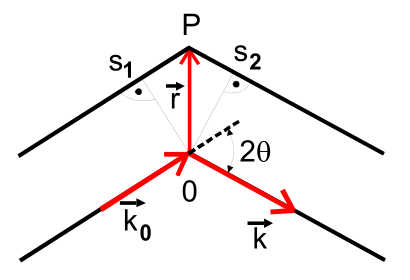
\includegraphics[width=0.5\linewidth]{images/phase.png}
    \caption{Skizze zur Berechnung der Phasenunterschiedes zweier Wellen, die an den Punkten O und P gestreut werden \cite{V41}.}
    \label{fig:phase}
\end{figure}

Für den einfallenden Wellenzahlvektor $\vec{k}_0$ und den Wellenzahlvektor $\vec{k}$ der gestreuten Welle gilt
\begin{equation*}
    |\vec{k}| = |\vec{k}_0| = \frac{1}{\lambda}\,,
\end{equation*}
woraus sich für den Gangunterschied $\Delta s$
\begin{equation*}
    \Delta s = s_1 + s_2 = \vec{r} \cdot \left(\frac{\vec{k}}{k} - \frac{\vec{k}_0}{k_0}\right)\,,
\end{equation*}
ergibt.
Somit ist der Phasenunterschied $\Delta \phi$
\begin{equation*}
    \Delta \phi = 2 \pi \frac{\Delta s}{\lambda} = 2 \pi \vec{r} \cdot \left(\vec{k} - \vec{k}_0\right)\,,
\end{equation*}
womit sich der Atomformfaktor als Fouriertransformierte der Ladungsverteilung $\rho$ durch
\begin{equation*}
    f = \int_\text{Hülle} e^{-i \Delta \phi} \rho(\vec{r}) \mathrm{d}^3r = \int_\text{Hülle} e^{-i 2 \pi \vec{r} \cdot \left(\vec{k} - \vec{k}_0\right)} \rho(\vec{r}) \mathrm{d}^3r\,,
\end{equation*}
bestimmen lässt.
\\
Wird nun die Streuung an mehreren Atomen einer Elementarzelle betrachtet, so treten auf Grund des festen Abstandes der Atome zueinander Interferenzeffekte auf.
Die Berechnung des Phasenunterschieds erfolgt analog zu der Streuung an zwei Elektronen mit dem Abstand $\vec{r}_j$ zwischen zwei Atomen
\begin{equation*}
    \Delta \phi = 2 \pi \vec{r}_j \cdot \left(\vec{k} - \vec{k}_0\right)\,.
\end{equation*}
Für die Streuamplitude $A$ der gesamten Elementarzelle muss nun über alle Atome innerhalb der Zelle phasenrichtig summiert werden
\begin{equation*}
    A = \sum_j f_j e^{-2 \pi i \vec{r}_j \cdot \left(\vec{k} - \vec{k}_0\right)} I_e = \sum_j f_j e^{-2 \pi i \left(x_j\vec{a} + y_j\vec{b} + z_j\vec{c}\right) \cdot \left(\vec{k} - \vec{k}_0\right)} I_e := S\,.
\end{equation*}
S beschreibt somit die Strukturamplitude der Elementarzelle.
Der Streuwinkel berechnet sich über
\begin{equation*}
    |\vec{k} - \vec{k}_0| = \frac{2 \sin{\Theta}}{\lambda}\,.
\end{equation*}
\\
Trifft die einfallende Strahlung als ebene Welle auf den Kristall, treten konstruktive Interferenzen zwischen benachbarten Netzebenen nur dann auf, wenn ihr Gangunterschied $\Delta s$ ein ganzzahliges Vielfaches der Wellenlänge $\lambda$ ist.
Mithilfe der Abbildung \ref{fig:bragg} und den Zusammenhängen
\begin{align*}
    \alpha_1 + \alpha_2 &= \pi - 2 \Theta\,,\\
    \frac{\pi}{2} - \Theta &= \alpha_2 + \beta\,,
\end{align*}
folgt für
\begin{align*}
    t \cdot \left(\cos{\alpha_1} + \cos{\alpha_2}\right) = 2 t \cos{\beta} \cos{\Theta}\,.
\end{align*}
\begin{figure}[h!]
    \centering
    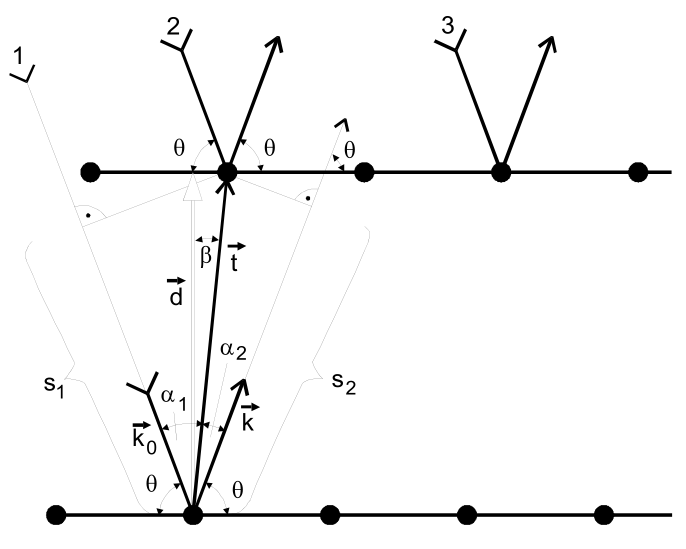
\includegraphics[width=0.5\linewidth]{images/bragg.png}
    \caption{Skizze zur Ableitung der Braggschen Bedingung \cite{V41}.}
    \label{fig:bragg}
\end{figure}

Somit ergibt sich die Braggsche Bedingung
\begin{equation*}
    n\lambda = 2 d \sin{\Theta} \qquad n \in \mathbb{N}_{>0}\,.
\end{equation*}
mit dem Netzebenenabstand $d$.

Betrachtet man die reziproken Gittervektoren
\begin{align*}
    \vec{A} = \frac{\vec{b} \times \vec{c}}{\vec{a}\cdot\left(\vec{b} \times \vec{c}\right)}\,,\\
    \vec{B} = \frac{\vec{c} \times \vec{a}}{\vec{a}\cdot\left(\vec{b} \times \vec{c}\right)}\,,\\
    \vec{C} = \frac{\vec{a} \times \vec{b}}{\vec{a}\cdot\left(\vec{b} \times \vec{c}\right)}\,,
\end{align*}
und den reziproken Gittervektor $\vec{g}$
\begin{equation*}
    \vec{g} = \vec{k} - \vec{k}_0 = h\vec{A} + k\vec{B} + l\vec{C}\,,
\end{equation*}
ergibt sich für die Streuamplitude $S$
\begin{equation*}
    S = \sum_j f_j e^{-2 \pi i \vec{r}_j \vec{g}} = \sum_j f_j e^{-2 \pi i \left(x_j h + y_j k + z_j l\right)}\,.
\end{equation*}
Somit ist es möglich, dass kein Reflex stattfindet, obwohl sich ein Braggscher Winkel berechnen lässt.

\section{Aufbau und Durchführung} % (fold)
\label{sub:debye_scherrer_verfahren}

\begin{figure}[h!]
    \centering
    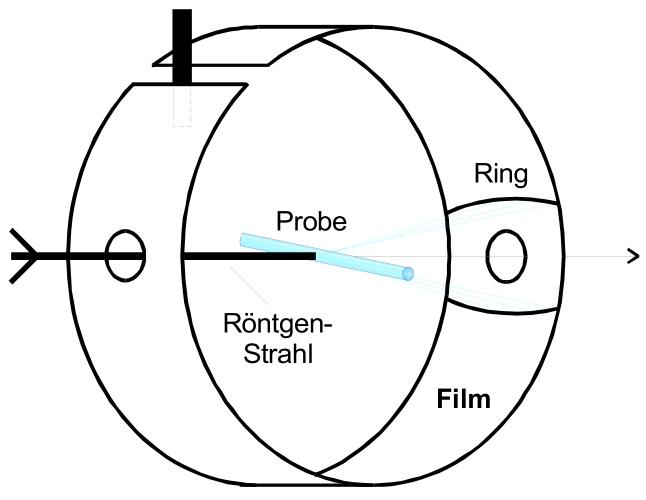
\includegraphics[width=0.5\linewidth]{images/aufbau.png}
    \caption{Schematischer Aufbau zur Herstellung einer Debye-Scherrer-Aufnahme \cite{V41}.}
    \label{fig:aufbau}
\end{figure}
In Abbildung \ref{fig:aufbau} ist der Messaufbau schematisch dargestellt.
Um die Größe und Gestalt der Elementarzelle des Probenmaterials zu bestimmen, wird die Probe mit monochromatischem Röntgenlicht bestrahlt und die Beugungswinkel $\Theta$ der auftretenden Bragg-Reflexe gemessen.
Um ein möglichst genaues Signal zu erhalten, wird das Debye-Scherrer-Verfahren verwendet.
Bei diesem wird eine fein pulverisierte, kristalline Probe auf einen dünnen Zylinder aufgebracht, sodass die Orientierung der Mikrokristalle statistisch über den ganzen Raumwinkel verteilt sind.
Somit ist die Wahrscheinlichkeit groß, einige Kristallite in Reflexionsstellug zu finden.
Um die Wahrscheinlichkeit noch weiter zu vergrößern, wird die Probe zudem während des Bestrahlens um die Längsachse gedreht.
\\
Bei der Messung kommt es zu systematischen Fehlern.
Dies hat zur Folge, dass die Gitterkonstante $a$ eine scheinbare Abhängigkeit vom Winkel $\Theta$ aufweist.
Dies ist im wesentlichen auf zwei Effekte zurückzuführen.
\begin{figure}[h!]
    \centering
    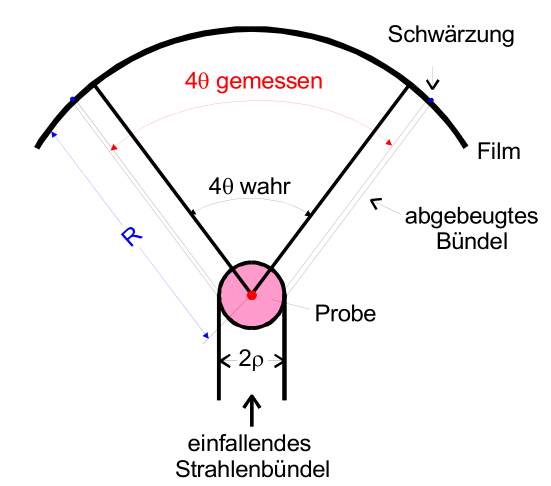
\includegraphics[width=0.5\linewidth]{images/fehler1.png}
    \caption{Auftretender systematischer Fehler bei der $\Theta$ Bestimmung infolge der Absorption furch die Probe \cite{V41}.}
    \label{fig:fehler1}
\end{figure}
Wie in Abbildung \ref{fig:fehler1} dargestellt, findet eine nahezu vollständige Absorption des Strahls an der Probe statt, sodass nur an einem schmalen Streifen des Zylinders eine Beugung stattfindet.
Somit wird der Winkel $4\Theta$ zu groß gemessen, sodass an der Gitterkonstanten $a$ die Korrektur $\Delta a_A$ über
\begin{equation*}
    \frac{\Delta a_A}{a} = \frac{\rho}{2R} \left(1-\frac{R}{F}\right) \frac{\cos^2{\Theta}}{\Theta}\,,
\end{equation*}
mit $\rho$ als dem Probenradius, $R=\SI{57.3}{\milli\meter}$ dem Kameraradius und $F=\SI{130}{\milli\meter}$ dem Abstand Fokus-Probe, angewendet werden muss.

\begin{figure}[h!]
    \centering
    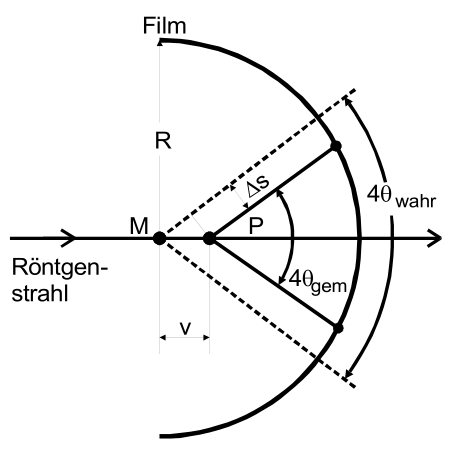
\includegraphics[width=0.5\linewidth]{images/fehler2.png}
    \caption{Auftretender systematischer Fehler bei der $\Theta$ Bestimmung infolge der Verschiebung der Probenachse gegen die Achse des Filmzylinders \cite{V41}. (M = Durchstoßpunkt der Filmzylinderachse durch die Zeichenebene, P = Durchstoßpunkt der Probenachse)}
    \label{fig:fehler2}
\end{figure}
Weiterhin kann es passieren, dass die Probenachse nicht mit der Achse des Filmzylinders zusammenfällt.
Wie in Abbildung \ref{fig:fehler2} angedeutet, ergibt sich ein Winkelfehler von
\begin{equation*}
    \Delta \Theta = \frac{v}{R}\cos{\Theta}\sin\Theta\,,
\end{equation*}
mit $v=\overline{MP}$.
Somit ist eine Korrektur der Form
\begin{equation*}
    \frac{\Delta a_V}{a} = \frac{v}{R}\cos^2{\Theta}\,,
\end{equation*}
nötig.

Näherungweise gilt
\begin{equation*}
    \Delta a_\text{ges} = \Delta a_V + \Delta a_A \propto \cos^2{\Theta}\,,
\end{equation*}
sodass die Gitterkonstante $a$ durch eine lineare Regression bestimmt werden kann.
\\
Im ersten Teil des Versuchs wird durch Ausmessen der Radien der Beugungswinkel berechnet und der Netzebenabstand $d$ bestimmt.

Im zweiten Teil wird die Kristallstruktur den Reflexen zugeordnet und abschließend die Gitterkonstante der Struktur bestimmt.
